
% ---
% Arquivo com a metodologia do Trabalho de Conclusão de Curso do aluno
% Daniel Noriaki Kurosawa
% da Escola Politécnica da Universidade de São Paulo
% ---
	% ---
	\chapter{Metodologia}\label{cap-metodologia}
	% ---
	
	Este capítulo apresenta o método de trabalho adotado para a execução das atividades
	do projeto e divide-se em três partes: organização de tarefas, escolha de hardware e software utilizados.
	
	

	
	% ---
	\section{Planejamento}\label{sec-planejamento}
	% ---
	Inicialmente, foi elaborado um diagrama de Gantt do sistema contendo as principais etapas do projeto (\autoref{fig_gantt}) a partir do qual foram identificadas as tarefas a serem realizadas durante o projeto, que foram posteriormente transferidas para o Trello.
	\begin{figure}[h!]
	\caption{\label{fig_gantt} Diagrama de Gantt do sistema }
		\begin{center}
	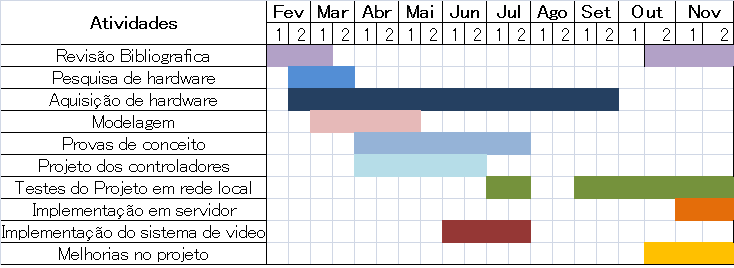
\includegraphics[width=\textwidth]{gantt.png}	
\end{center}
	\legend{Fonte: Autor}
\end{figure}

	% ---
	\subsection{Trello}\label{subsec-eap}
	% ---
	Trello é uma ferramenta de organização de projetos  baseada nos quadros Kanban da metodologia ágil. Extremamente versátil, permite uma análise rápida da situação do projeto, das etapas cumpridas e do cronograma geral do projeto. No Trello, é possível criar “boards” que agrupam listas (“lists”) de tarefas que devem ser feitas. Cada tarefa é então representada por um “card”, criado dentro de uma “list”. As “lists” criadas dentro da “board” do projeto são:\par
	
	\subparagraph{Backlog}: Tarefas que ainda precisam ser analisadas e aprovadas para serem colocadas na fase de atividades.
	\subparagraph{Sprint}: Tarefas a serem realizadas após a conclusão das tarefas sendo trabalhadas atualmente.
	\subparagraph{Doing}: Tarefas em execução.
	\subparagraph{To be verified}: Tarefas executadas a serem revisadas.
	\subparagraph{Done}: Tarefas terminadas.
	\subparagraph{Halt}: Tarefas suspensas/canceladas.

		\begin{figure}[h!]
		\caption{\label{fig_trello} Kanban do projeto usando Trello }
		\begin{center}
	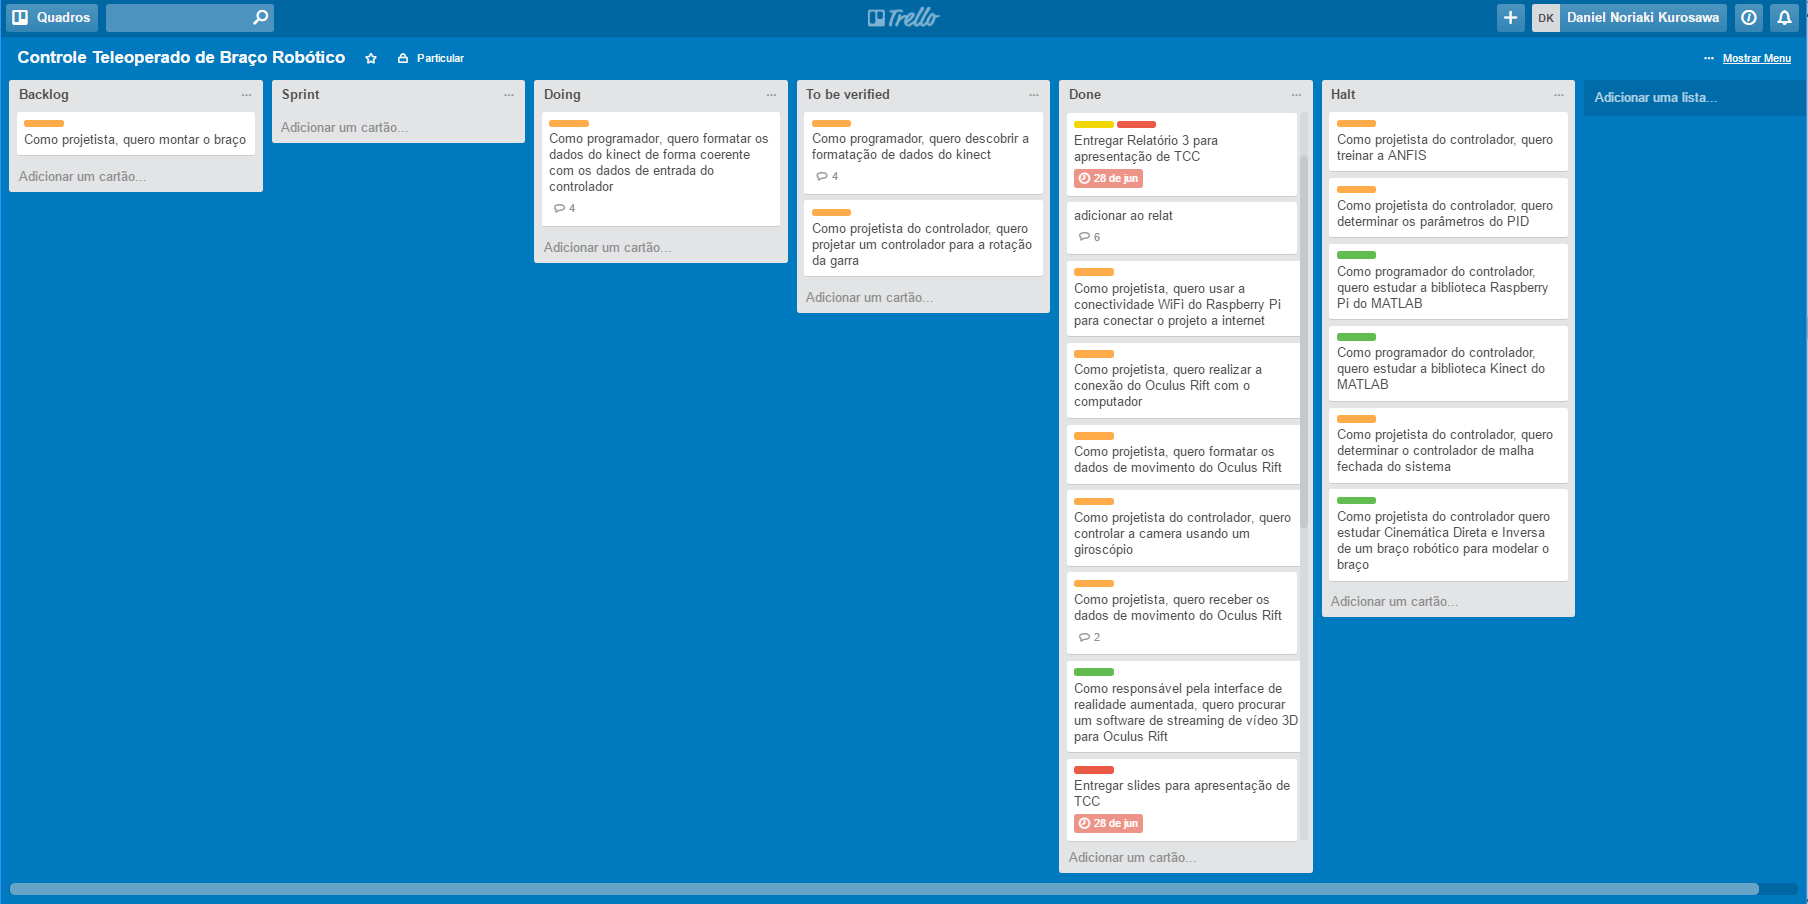
\includegraphics[width=\textwidth]{trello.png}	
	\end{center}
	\legend{Fonte: Autor}
	\end{figure}
	
	
	% ---
	\subsection{Cronograma}\label{subsec-cronograma}
	% ---
	
	O cronograma do projeto foi planejado a partir dos pacotes de trabalho definidos na Estrutura Analítica de Projeto. Os participantes então fizeram reuniões para estimar o tempo, com a aplicação dessas estimativas a um calendário, considerando ainda as datas de entrega oficiais da disciplina. Com todas as estimativas feitas, o projeto tem a primeira e segunda fase com duração até o fim de Julho, com intuito de adiantar tanto a documentação quanto a implementação, como pode-se observar no diagrama de Gantt  \autoref{fig_gantt} abaixo.
	
	
	% ---
	\subsection{Requisitos}\label{subsec-requisitos}
	% ---
	
	Os requisitos foram divididos primeiramente em funcionais e não-funcionais. Além disso, existem outras divisões relacionadas a hardware, software, estética e módulos do sistema. Para cada requisito foi dado um peso, conforme avaliação da relevância deste requisito para este projeto, de modo que no topo da árvore haja uma soma equivalente a 1.
	
	% ---
	\subsubsection{Requisitos Funcionais}\label{subsubsec-requisitos-func}
	% ---
	
	\paragraph{Requisitos de hardware} 
	
	É importante observar que estes dividem-se entre a lamparina, que serve de ponto de acesso, e o módulo de celular, com pesos iguais entre os dois, já que a comunicação é bilateral e ambos têm importância equivalente. Há requisitos em comum entre esses subsistemas:
	

	\paragraph{Requisitos de software} 
	Dividem-se entre a lamparina, o módulo de celular e o aplicativo, utilizado para receber e enviar dados para este módulo. Existem requisitos que são complementares às funções de hardware, porém correspondentes às soluções de software adotadas, como a implementação da norma IEEE 802.15.7 e a comunicação full-duplex um a um. Além destes, existem os requisitos de software comuns tanto à lamparina, ou Access Point Li-Fi, como ao módulo de telefone:
	

	\subsubsection{Requisitos Não-Funcionais}\label{subsubsec-requisitos-nfunc}
	


	
	\paragraph{Conclusão}
	

	\section{Software}\label{sec-software}
	% ---
	
	Explica as escolhas feitas no aspecto do software do projeto.
	
